% Source: Notion page “3. 系统总体设计”. Generated without rewriting its content.
\chapter{系统总体设计}

\section{总体架构图}

\begin{figure}[htbp]
\centering
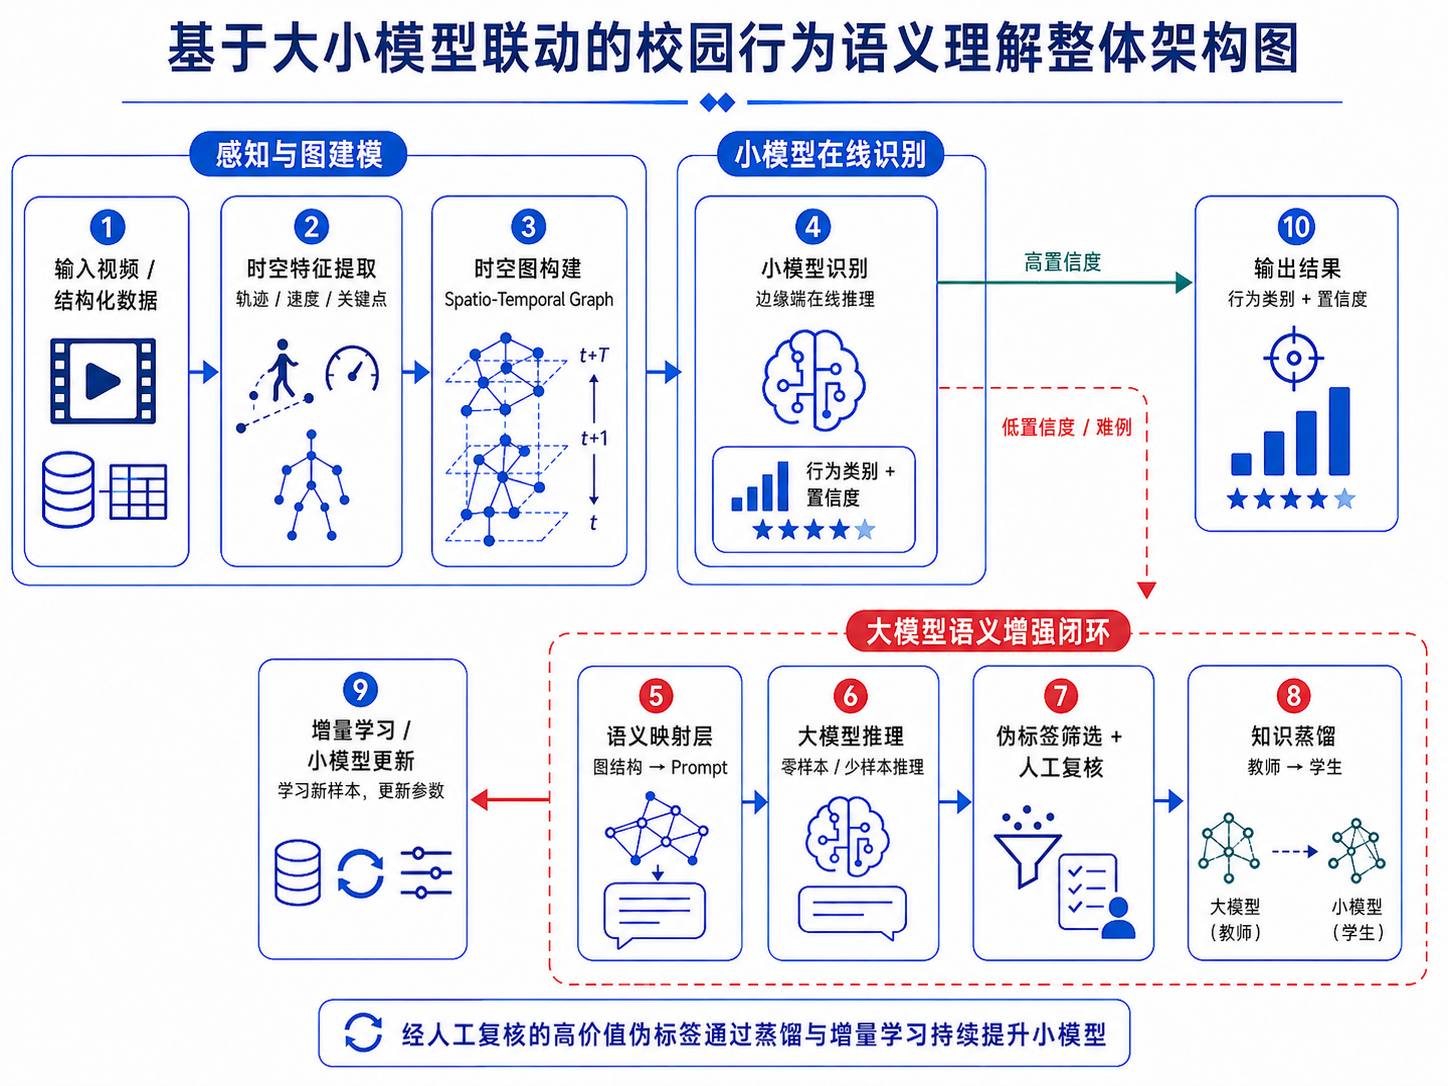
\includegraphics[width=0.96\linewidth,keepaspectratio]{figures/notion_image_01.png}
\end{figure}

\section{系统模块划分}

\begin{center}
\small
\begin{longtable}{|>{\raggedright\arraybackslash}p{0.46\linewidth}|>{\raggedright\arraybackslash}p{0.46\linewidth}|}
\hline
模块 & 功能 \\
\hline
数据输入模块 & 视频读取与预处理 \\
\hline
骨架提取模块 & 多人关键点检测 \\
\hline
小模型识别模块 & 六类行为分类 \\
\hline
语义映射模块 & 将骨架行为转换为语义信息 \\
\hline
大模型推理模块 & 细粒度行为语义判断 \\
\hline
协同决策模块 & 综合大小模型结果 \\
\hline
蒸馏模块 & 大模型知识迁移 \\
\hline
增量学习模块 & 新数据加入和模型升级 \\
\hline
可视化模块 & 展示识别结果 \\
\hline
\end{longtable}
\end{center}

